\section{Lognormal Distribution ($\text{Lognormal}(\mu ,\sigma ^{2})$)}

\begin{table}[H]
    \hfill
    \begin{minipage}{0.45\linewidth}
        \begin{figure}[H]
            \centering
            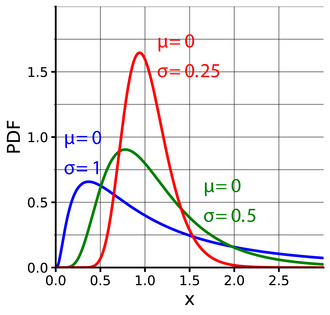
\includegraphics[
                width=\linewidth,
                height=5cm,
                keepaspectratio,
            ]{images/distributions/Log-normal-pdfs.png}
            \caption{Lognormal Distribution: PDF \cite{wiki/Log-normal_distribution}}
        \end{figure}
    \end{minipage}
    \hfill
    \begin{minipage}{0.45\linewidth}
        \begin{figure}[H]
            \centering
            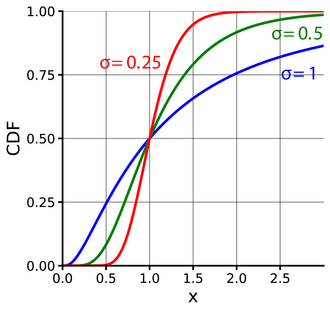
\includegraphics[
                width=\linewidth,
                height=5cm,
                keepaspectratio,
            ]{images/distributions/Log-normal-cdfs.png}
            \caption{Lognormal Distribution: CDF \cite{wiki/Log-normal_distribution}}
        \end{figure}
    \end{minipage}
    \hfill
\end{table}



\subsection{PDF}

\begin{enumerate}
    \item[] $
        f_{\mu, \sigma}(x) = \dfrac{1}{x\sigma \sqrt{2\pi}} \exp\dCurlyBrac{
            -\dfrac{(\log(x) - \mu)^2}{2\sigma^2}
        }
    $
    \hfill \cite{statistics/book/Statistics-for-Data-Scientists/Maurits-Kaptein}

    \item the lognormal PDF describes populations with positive values
    \hfill \cite{statistics/book/Statistics-for-Data-Scientists/Maurits-Kaptein}

    \item relative standard deviation  is constant for the lognormal PDF.
    This means that larger values demonstrate larger variability, but the ratio with variability is constant whether we observe smaller or larger values.
    \hfill \cite{statistics/book/Statistics-for-Data-Scientists/Maurits-Kaptein}

    \item the lognormal PDF is not symmetric like the normal PDF, which makes sense when values are limited from below, but not from above.
    \hfill \cite{statistics/book/Statistics-for-Data-Scientists/Maurits-Kaptein}

    \item  If the population values can be described by a lognormal PDF, the normal PDF would then describe the logarithmic transformation of the population values (using the natural logarithm).
    \hfill \cite{statistics/book/Statistics-for-Data-Scientists/Maurits-Kaptein}

    \item The parameters $\mu$ and $\sigma$ have a different meaning in the lognormal PDF than in the normal PDF.
    They do represent the population mean and standard deviation, but only for the logarithmic transformed values of the population.
    Their meaning in relation to the mean and standard deviation of the population values in the original scale is now more complicated.
    \hfill \cite{statistics/book/Statistics-for-Data-Scientists/Maurits-Kaptein}
\end{enumerate}



\subsection{Summary}

\begin{enumerate}
    \item \textbf{Notation}:
    ${\displaystyle \operatorname {Lognormal} \left(\mu ,\,\sigma ^{2}\right)}$
    \hfill \cite{wiki/Log-normal_distribution}

    \item \textbf{Parameters}:
    \begin{enumerate}
        \item ${\displaystyle \mu \in (-\infty ,+\infty )}$: logarithm of location
        \hfill \cite{wiki/Log-normal_distribution, statistics/book/Statistics-for-Data-Scientists/Maurits-Kaptein}

        \item ${\displaystyle \sigma >0}$: logarithm of scale
        \hfill \cite{wiki/Log-normal_distribution, statistics/book/Statistics-for-Data-Scientists/Maurits-Kaptein}
    \end{enumerate}

    \item \textbf{Support}: ${\displaystyle x\in (0,+\infty )}$
    \hfill \cite{wiki/Log-normal_distribution, statistics/book/Statistics-for-Data-Scientists/Maurits-Kaptein}

    \item \textbf{PDF}:
    ${\displaystyle {\dfrac {1}{x\sigma {\sqrt {2\pi }}}}\exp \left(-{\dfrac {\left(\ln x-\mu \right)^{2}}{2\sigma ^{2}}}\right)}$
    \hfill \cite{wiki/Log-normal_distribution, statistics/book/Statistics-for-Data-Scientists/Maurits-Kaptein}

    \item \textbf{CDF}:
    $
        {\displaystyle {{\dfrac {1}{2}}\left[1+\operatorname {erf} \left({\dfrac {\ln x-\mu }{\sigma {\sqrt {2}}}}\right)\right]
        =\Phi {\left({\dfrac {\ln x-\mu }{\sigma }}\right)}}}
    $
    \hfill \cite{wiki/Log-normal_distribution}

    \item \textbf{Quantile}:
    $
        {\displaystyle {\exp \left(\mu +{\sqrt {2\sigma ^{2}}}\operatorname {erf} ^{-1}(2p-1)\right)
        =\exp(\mu +\sigma \Phi ^{-1}(p))}}
    $
    \hfill \cite{wiki/Log-normal_distribution}

    \item \textbf{Mean}: ${\displaystyle \exp \left(\mu +{\dfrac {\sigma ^{2}}{2}}\right)}$
    \hfill \cite{wiki/Log-normal_distribution}

    \item \textbf{Median}: ${\displaystyle \exp(\mu )}$
    \hfill \cite{wiki/Log-normal_distribution}

    \item \textbf{Mode}: ${\displaystyle \exp \left(\mu -\sigma ^{2}\right)}$
    \hfill \cite{wiki/Log-normal_distribution}

    \item \textbf{Variance}:
    ${\displaystyle \left[\exp(\sigma ^{2})-1\right]\exp \left(2\mu +\sigma ^{2}\right)}$
    \hfill \cite{wiki/Log-normal_distribution}

    \item \textbf{Skewness}:
    ${\displaystyle \left[\exp \left(\sigma ^{2}\right)+2\right]{\sqrt {\exp(\sigma ^{2})-1}}}$
    \hfill \cite{wiki/Log-normal_distribution}

    \item \textbf{Excess kurtosis}:
    ${\displaystyle \exp \left(4\sigma ^{2}\right)+2\exp \left(3\sigma ^{2}\right)+3\exp \left(2\sigma ^{2}\right)-6}$
    \hfill \cite{wiki/Log-normal_distribution}

    \item \textbf{Entropy}: ${\displaystyle \log _{2}\left({\sqrt {2\pi e}}\,\sigma e^{\mu }\right)}$
    \hfill \cite{wiki/Log-normal_distribution}

    \item \textbf{Fisher information}:
    ${\displaystyle {\dfrac {1}{\sigma ^{2}}}{\begin{pmatrix}1&0\\0&2\end{pmatrix}}}$
    \hfill \cite{wiki/Log-normal_distribution}

    \item \textbf{Method of moments}:
    \begin{enumerate}
        \item ${\displaystyle \mu =\ln \operatorname {E} [X]-{\dfrac {1}{2}}\ln \left({\dfrac {\operatorname {Var} [X]}{\operatorname {E} [X]^{2}}}+1\right),}$
        \hfill \cite{wiki/Log-normal_distribution}

        \item ${\displaystyle \sigma ={\sqrt {\ln \left({\dfrac {\operatorname {Var} [X]}{\operatorname {E} [X]^{2}}}+1\right)}}}$
        \hfill \cite{wiki/Log-normal_distribution}
    \end{enumerate}

    \item \textbf{Expected shortfall}:
    $
        {\displaystyle {{\dfrac {e^{\mu +{\dfrac {\sigma ^{2}}{2}}}}{2p}}\left[1+\text{erf} \left({\dfrac {\sigma }{\sqrt {2}}}+\operatorname {erf} ^{-1}(2p-1)\right)\right]
        ={\dfrac {e^{\mu +{\dfrac {\sigma ^{2}}{2}}}}{1-p}}\left[1-\Phi (\Phi ^{-1}(p)-\sigma )\right]}}
    $
    \hfill \cite{wiki/Log-normal_distribution}

    \item \textbf{Relative Standard Deviation}: $\sqrt{\exp\dCurlyBrac{\sigma^2} - 1}$
    \hfill \cite{statistics/book/Statistics-for-Data-Scientists/Maurits-Kaptein}
    \\
    (RSD = standard deviation divided by the mean)
    \hfill \cite{statistics/book/Statistics-for-Data-Scientists/Maurits-Kaptein}
\end{enumerate}





